\documentclass[a4paper,oneside,reqno]{amsart}

\input{../../../../cambridge-macros.tex}

%    Set assignment information here
\newcommand{\authorname}{Feynman Liang}
\newcommand{\coursename}{MLSALT5: Speech and Language Processing Applications}
\newcommand{\assignmentname}{Practical: Keyword Spotting}

\begin{document}

\title{\coursename\\\assignmentname}

\author{\authorname}
\date{\today}

\maketitle

\section{Introduction}

This practical investigates keyword spotting (KWS) with written (i.e.\ manually
transcribed) queries on low resource languages. Specifically, we use a Swahili
corpus from the IARPA Babel project's 2015 surprise evaluation language. We
implement an \emph{efficient} KWS system which can perform \emph{constant time
queries for individual terms} and only requires time linear in the 1-best list
size to construct the KWS index from 1-best ASR outputs. To allow for
\emph{queries containing OOV terms}, we support morphological
decomposition\cite{narasimhan2014morphological} of both the index and the
query.

Additionally, we use outputs from a WFST-based KWS system provided by
IBM\cite{gales2014speech} to quantify the performance impact of using 1-best
lists instead of full word lattices and investigate \emph{system combination}
using CombSUM\cite{lee1997analyses}.  While combining hits and their scores
from multiple systems, the issue of \emph{score normalization} naturally
arises. We implement sum-to-one (STO) normalization\cite{mamou2013system} and
study how it affects system combination performance.

\section{1-best keyword spotting}

\subsection{Word based KWS}

We implement a word-based KWS system in \texttt{KWSIndex}. Using a 1-best ASR
decoding output with posterior scores, we build an inverted index mapping
individual terms to their respective occurrence time-spans and scores.

The inverted index is implemented using a hashmap, which enable insertion and
lookup operations with $O(1)$ amortized time complexity. Each term in the
1-best output is inserted into the index, so constructing the index requires
time linear in the size of the 1-best list. Querying the index with an individual
term corresponds to a hashmap lookup and hence can be efficiently performed in
constant-time.

For queries containing a sequence of $N$ terms (i.e.\ phrase queries), we first
query each term individually to obtain a sequence of collections of term hits.
Letting $\{k_1, \ldots,k_N\}$ denote the number of hits for each term, we can
view this sequence of collections of term hits as a $N$-layer lattice with $k_i$
nodes in each layer.  Next, we extract phrase hits using the constraints that
any valid phrase hit must satisfy:
\begin{enumerate}
  \item All term hits in the sequence are from the same file
  \item The time between terms should be $\leq 0.5$ seconds
  \item To prevent phrase matches which skip words having duration $\leq 0.5$, contiguous
    words in a phrase hit should have equal end/start times
\end{enumerate}
This operation corresponds to finding paths through the network. We take the
average score of all term hits in a phrase query to be the score of the phrase
hit and the min/max of the start/end times over the individual terms to be
the start/end time of the phrase hit.

Querying phrases is implemented using \texttt{map} and \texttt{reduce} % TODO: easily parallelize
operations in the \texttt{KWSIndex.get} method. Obtaining the hits for each
individual term requires $O(N)$ time. In the worst case, all paths through the
lattice are valid so computing all phrase hits requires $O(\prod_{k=1}^N k_i)$
time. However, in practice this cost is much less since each term hit is
usually only part of a few phrase hits. Furthermore, techniques such as beam
search can be used to mitigate computational cost of this lattice search.

\subsubsection{Experimental results}

In \autoref{tab:word} we report the maximum term-weighted values (MTWV) attained
from running our word-based KWS system on the reference transcription
(\texttt{reference.ctm}) and provided 1-best word decoding
(\texttt{decode.ctm}).

\begin{table}[ht!]
  \begin{tabular}{clc}
    \toprule
    System & & MTWV \\
    \midrule
    \multirow{3}{*}{Word (\texttt{reference.ctm})}
      & IV & 1.000 \\
      & OOV & 1.000 \\
      & All & 1.000 \\
    \multirow{3}{*}{Word (\texttt{decode.ctm})}
      & IV & 0.402 \\
      & OOV & 0.000 \\
      & All & 0.300 \\
    \bottomrule
  \end{tabular}
  \caption{Performance of 1-best word-based KWS}
  \label{tab:word}
\end{table}

As expected, our system achieves 1.000 MTWV on the reference transcription.
The performance on 1-best ASR outputs is significantly worse. This is primarily
due to two effects:
\begin{enumerate}
  \item ASR transcription errors, which results in deterioration of performance on IV queries.
  \item Lack of support for OOV terms, which results in all queries containing OOV
    terms to yield no hits and a $0.000$ MTWV.
\end{enumerate}

\subsection{Morphological Decomposition}

One method to improve the poor performance on OOV query terms is to perform
morphological decomposition on both the index and query
terms\cite{narasimhan2014morphological}. Since different terms may have the
same morphological decomposition, hits for OOV query terms can be found if its
morphological decomposition coincides with the decomposition of an IV term.

\texttt{MorphDecompose} uses morph dictionaries for the decoding vocabulary
(\texttt{morph.dct}) and the query terms (\texttt{morph.kwslist.dct}) to
perform morphological decomposition of terms and phrases. When decomposing a
single term hit into multiple morph hits, we divide the occurrence time-span of
the term equally among the constituent morphs and choose the morph hits'
scores to be equal to the term hit's score. This ensures that the duration and
score for an individual term remains the same before and after decomposition.

In \texttt{KWSIndexMorph}, we use \texttt{MorphDecompose} to decompose queries
at runtime.  We also decompose the KWS index at initialization if required
(e.g.\ when using the word-based ASR output \texttt{decode.ctm} instead of the
morph-based \texttt{decode-morph.ctm}).

After decomposition, term and phrase queries are handled almost identically to
\texttt{KWSIndex.get}. A \emph{notable exception is due to a bug in the
supplied IBM morph segmentation}, which contains overlapping morph
segmentations. For example, in \texttt{decode-morph.ctm}:
\begin{lstlisting}[firstnumber=101748]
BABEL_OP2_202_90080_20140319_222809_inLine 1 396.14 0.26 pia 0.929472
BABEL_OP2_202_90080_20140319_222809_inLine 1 396.14 1.98 pia 0.178492
\end{lstlisting}
Notice that both entries have start time $396.14$ and hence overlap.
This means that the decoding outputs are no longer disjoint. To mitigate
this problem, we relax the contiguity requirement (i.e.\ end/start times between
consecutive words in a phrase hit are equal) when returning hits.

\subsubsection{Experimental results}

\autoref{tab:morph} reports our results using morphological decomposition.
The Morph system performs morph decomposition on a word-based ASR's 1-best
decoding while the Morph.MD system directly uses a morph-based ASR's 1-best
output to construct the KWS index.

\begin{table}[ht!]
  \begin{tabular}{clc}
    \toprule
    System & & MTWV \\
    \midrule
    \multirow{3}{*}{Morph (\texttt{decode.ctm})}
      & IV & 0.378 \\
      & OOV & 0.016 \\
      & All & 0.304 \\
    \multirow{3}{*}{Morph.MD (\texttt{decode-morph.ctm})}
      & IV & 0.373 \\
      & OOV & 0.065 \\
      & All & 0.310 \\
    \bottomrule
  \end{tabular}
  \caption{Performance of 1-best KWS with morphological decomposition}
  \label{tab:morph}
\end{table}

Notice that performance on OOV queries is no longer $0$, indicating that
morph decomposition has allowed the system to resolve some OOV queries.
Morph.MD appears to handle OOV words better than Morph, possibly because
the ASR system itself was built directly on morph targets. However, this
only happens when the morph decomposition of the query term coincides
with an IV morph decomposition hence the gap between IV and OOV queries
is still large.

In addition, the MTWV for IV terms has slightly degraded compared to the
word-based KWS system. To understand why, recall that TWV is computed as
\begin{align}
  \label{eq:twv}
  TWV = 1 - (P_{miss} + \beta P_{FA})
\end{align}
where $\beta = 999.9$ for the Babel project's
evaluation\cite{wang2014depth}.  In particular, note that false positives
($P_{FA}$) significantly hurt the TWV metric. In the morph based systems, when
two different terms share the same morph decomposition the hits for both will
be returned when either is queried.  Additionally, relaxation of the contiguity
constraint for phrase queries to work around the IBM segmenter's bug leads to
an increase in the number of valid phrase hits. Both factors increase the
number of false positives when using \texttt{KWSIndexMorph}, which we confirm
in the \#FA column of \autoref{tab:morph-word-perf}.

\begin{table}
  \begin{tabular}{cccccc}
    \toprule
    System                            & \#Sys & \#CorDet & \#FA & \#Miss\\
    \midrule
    Word (\texttt{decode.ctm})        & 725   & 405      & 320  & 558\\
    Morph (\texttt{decode.ctm})       & 1308  & 420      & 888  & 543\\
    Morph.MD (\texttt{decode-morph.ctm}) & 1230  & 415      & 815  & 548\\
    \bottomrule
  \end{tabular}
  \caption{Detailed performance metrics for word vs morph based KWS}
  \label{tab:morph-word-perf}
\end{table}

\subsection{Score normalization}

TWV (\autoref{eq:twv}) is proportional to $P_{miss}$ and hence inversely
proportional to the frequency of a term. In other words, the TWV metric
emphasizes recall of rare terms\cite{mamou2013system}. However, the scores
from the ASR output represent posterior probabilities and do not capture
this emphasis on more rare terms.

Another problem with using raw scores is that they correspond to the posterior
probabilities \emph{of a particular ASR system}. Hence, scores may not be
comparable across different systems. This becomes especially important when
combining the hits from multiple systems\cite{mamou2013system}.

Various methods for addressing these concerns have been proposed. In this practical,
we explore sum-to-one normalization, which has been shown to yield significant
improvements in TWV\cite{gales2014speech}. In STO normalization, the score
$s_{ki}$ for the $i$th hit for keyword $k$ is adjusted according to
\begin{align}
  \label{eq:sto}
  \hat{s}_{ki} = \frac{s_{ki}}{\sum_{j \in \{\text{hits for $k$}\}} s_{kj}}
\end{align}
The denominator is the sum of the posterior estimates for all hits and represents
an approximate number of occurrences for the query. For rare terms, this quantity
will be lower and hence the normalized score will be higher and more likely to be
above the decision threshold\cite{mamou2013system}.

Although not investigated in this practical, another method for explicitly
emphasizing rare terms is to use keyword specific thresholds (KST) which are lower
for rare terms and higher for common terms. Experiments have shown that KST and STO
both yield comparable results\cite{wang2014depth}.


% TODO: discuss QL and Discriminative

We implement STO normalization in \texttt{QueryResult}, the class for results
returned by a \texttt{KWSIndex}.

\subsubsection{Experimental results}

In \autoref{tab:sto}, we compare the MTWV of the systems with and without STO
score normalization. The Threshold column is the decision threshold attaining
the MTWV.

\begin{table}[ht!]
  \begin{tabular}{ccccc}
    \toprule
    System                                & Threshold & IV    & OOV   & All \\
    \midrule
    Word (\texttt{decode.ctm})            & 0.167     & 0.402 & 0.000 & 0.320 \\
    Morph (\texttt{decode.ctm})           & 0.205     & 0.378 & 0.016 & 0.304 \\
    Morph (\texttt{decode-morph.ctm})     & 0.301     & 0.373 & 0.065 & 0.310 \\
    \hline
    Word STO (\texttt{decode.ctm})        & 0.029     & 0.402 & 0.000 & 0.320 \\
    Morph STO (\texttt{decode.ctm})       & 0.056     & 0.391 & 0.015 & 0.314 \\
    Morph STO (\texttt{decode-morph.ctm}) & 0.047     & 0.389 & 0.065 & 0.323 \\
    \bottomrule
  \end{tabular}
  \caption{Best possible TWVs for systems with vs without sum-to-one (STO) score normalization}
  \label{tab:sto}
\end{table}

Notice that the best decision threshold decreases after applying STO. This is
because the denominator in STO (\autoref{eq:sto}) is a sum of posterior scores,
which represent an approximate number of occurrences for the query and hence
usually $\geq 1$.

In general, applying STO improves TWV performance. For both the morph-based KWS
systems, gains of $0.010$ and $0.013$ in overall TWV were observed for the
\texttt{decode.ctm} and \texttt{decode-morph.ctm} systems respectively.  These
gains are much smaller than the gains of $20\%$ reported in
\cite{mamou2013system}, likely because the authors are using full lattice
outputs whereas we are using $1$-best ASR outputs. %TODO: lattices give more alternativehypotheses

\section{System Combination}

Combining outputs from a diverse collection of systems is known to improve
performance by up to $14\%$\cite{mamou2013system}. Hence, we investigate system
combinations involving outputs from three different KWS systems with
unnormalized scores (a morph-based system Morph and two word-based systems
Word and Word Sys2) supplied by IBM. These systems utilize a WFST
approach and are run on full word-lattices instead of 1-best lists.

\subsection{STO normalization on individual IBM WFST outputs}

We first consider the provided outputs in isolation. \autoref{tab:ibm-indiv}
reports MTWV before and after STO normalization.

\begin{table}[ht!]
  \begin{tabular}{clcc}
    \toprule
    KWS System                 &     & Unnormalized & STO \\
    \midrule
    \multirow{3}{*}{Word}      & IV  & 0.501 & 0.579\\
                               & OOV & 0.000 & 0.000\\
                               & All & 0.309 & 0.460\\
                               \hline
    \multirow{3}{*}{Word Sys2} & IV  & 0.507 & 0.585\\
                               & OOV & 0.000 & 0.000\\
                               & All & 0.403 & 0.465\\
                               \hline
    \multirow{3}{*}{Morph}     & IV  & 0.430 & 0.556\\
                               & OOV & 0.089 & 0.367\\
                               & All & 0.360 & 0.520\\
    \bottomrule
  \end{tabular}
  \caption{STO score normalization applied to IBM KWS outputs.}
  \label{tab:ibm-indiv}
\end{table}

Just like \autoref{tab:word} and \autoref{tab:morph}, we see that prior to STO
the OOV performance is $0$ for the word-based systems and small for morph-based
systems.  However, the IV performance of the WFST-based systems are
significantly higher.  This is because these systems can utilize the full word
lattice, which encodes alternative hypotheses that can mitigate transcription
errors present in the highest-scoring transcription.

Unlike \autoref{tab:sto}, STO dramatically affects the performance of these
systems with overall TWV gains ranging from $0.061$ to $0.160$. These gains are
consistent with those reported in \cite{mamou2013system}. Since the WFST-based
system uses the full word-lattice, the consideration of alternative hypotheses
lead to a greater number of potential hits for any given query. Hence, we
expect more hits on average than when using 1-best decodings and therefore the
denominator in STO (\autoref{eq:sto}) is greater on average. As the average
term is more suppressed by STO normalization, the difference in normalized
score between rare and common terms is greater when using WFST-based outputs
and hence the effects of STO are more pronounced.

The significant $16\%$ improvement in Morph is largely due to a $27.8\%$
improvement on OOV terms. This suggests that the Morph system is capable of
spotting a large number of OOV queries, but also generates a lot of false
positives which lower the overall TWV\. After STO, the scores of the rare
terms are boosted relative to common ones, reducing the number of false
positives (i.e. $P_{FA}$ in \autoref{eq:twv}) and improving TWV.

\subsection{Combining multiple outputs}

Numerous methods for combining the outputs of multiple systems have been
proposed. In all methods we consider, the hits from two different systems are
merged if their occurrence time-spans overlap. The resulting combined hit's
start time and duration are set equal to the highest scoring. For combining
scores, \cite{soto2014comparison} evaluates a variety of methods and show that
CombSUM and CombMNZ offer good performance for KWS\. CombSUM sets the score of
the combined hit to be equal to the sum of all hits combined. CombMNZ modifies
CombSUM by multiplying the summed score with the number of hits in the combined
query. \cite{mamou2013system} uses a weighted form of CombMNZ (WCombNZ) where
each system is weighted by a coefficient proportional to that system's MTWV
prior to summation.

Since \cite{soto2014comparison} report similar performance for CombSUM and
CombMNZ and \cite{belkin1995combining} report superior performance for CombSUM,
we choose to implement CombSUM in the \texttt{ResultsCombiner} class. The
results from two systems are first unioned and then hits with overlapping
occurrence time-spans are grouped together to produce the combined output.

\begin{table}[ht!]
  \begin{tabular}{clc}
    \toprule
    Methodology & & MTWV \\
    \midrule
    \multirow{3}{*}{CombSUM.IBM}         & IV  & 0.493 \\
                                         & OOV & 0.086 \\
                                         & All & 0.410 \\
    \hline
    \multirow{3}{*}{STO-CombSUM.IBM}     & IV  & 0.601 \\
                                         & OOV & 0.364 \\
                                         & All & 0.552 \\
    \hline
    \multirow{3}{*}{CombSUM.IBM-STO}     & IV  & 0.590 \\
                                         & OOV & 0.369 \\
                                         & All & 0.545 \\
    \hline
    \multirow{3}{*}{STO-CombSUM.IBM-STO} & IV  & 0.601 \\
                                         & OOV & 0.366 \\
                                         & All & 0.553 \\

    \hline
    \multirow{3}{*}{STO-CombSUM.All-STO} & IV  & 0.596 \\
                                         & OOV & 0.366 \\
                                         & All & 0.549 \\
    \bottomrule
  \end{tabular}
  \caption{Normalization and system combination. ``STO-'' prefix denotes
  normalization of scores before combination, ``-STO'' suffix denotes normalization
  after combination, CombSUM.IBM is the combination of all three IBM systems,
  CombSUM.ALL is the combination of all three IBM systems with our word and
  morph-based KWS systems.}
  \label{tab:comb}
\end{table}

Our results are reported in \autoref{tab:comb}. We see that applying STO is
extremely important during system combination, with the normalized systems
achieving $13-14\%$ better performance than the unnormalized systems. Because
scores from different ASR systems are not directly comparable, an ASR system
with few alternative hypotheses will yield higher posterior scores and hence
without normalization will dominate the combination. However, the performance
is similar regardless whether STO is applied before (STO-CombSUM.IBM) or after
(CombSUM.IBM-STO) combination, suggesting that the majority of the improvement
comes from STO's increased emphasis on rare terms.

We found that \emph{the best performing system is STO-CombSUM.IBM-STO},
achieving MTWV of $0.553$. The DET curve for this system is shown in
\autoref{fig:det}.  It shows that the MTWV threshold of $0.0992$ yields $P_{FA}
\approx 0.006 \%$ and $P_{Miss} \approx 39\%$. The significantly lower $P_{FA}$
relative to $P_{Miss}$ is due to the Babel project's specification of $\beta =
999.9$ in \autoref{eq:twv}.

\begin{figure}[ht!]
  \begin{center}
    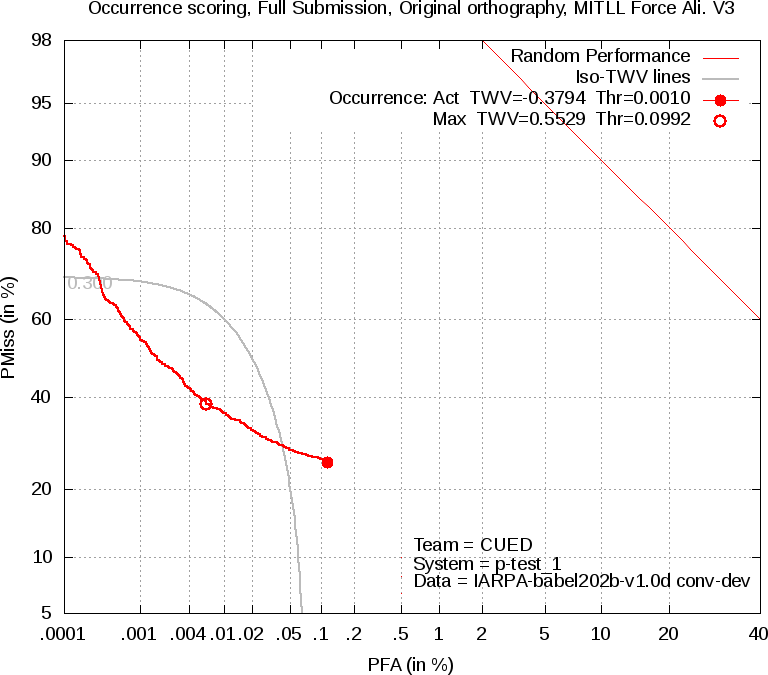
\includegraphics[scale=0.5]{Figures/sto-combSUM-det.png}
  \end{center}
  \caption{DET curve for STO-CombSUM.IBM-STO}
  \label{fig:det}
\end{figure}

Despite STO-CombSUM.All-STO utilizing outputs from our 1-best KWS systems in
addition to all the IBM outputs, it is still outperformed by
STO-CombSUM.IBM-STO . This is likely due to our worse performing 1-best KWS
outputs receiving the same weight as the better performing IBM outputs during
CombSUM.  To solve this, we could use a weighted combination method such as
WCombMNZ\cite{mamou2013system}.

\subsection{Impact of query length}

We also consider how the length of a query affects KWS system performance. The
\texttt{LengthMap} class generates a \texttt{.map} file mapping queries to
their lengths.  \texttt{scripts/termselect.sh} is then used with this
\texttt{.map} file to produce TWV scores segmented by query length.

\autoref{tab:query-length} compares the performance of various KWS systems on
different query lengths. In general, all systems appear to perform best on
queries of intermediate length ($2-4$). The improvements due to STO are more
significant than those due to system combination on all query lengths, but STO
is particularly helpful for shorter queries while system combination benefits
longer queries more. These observations are consistent with those found in
\cite{mamou2013system}.

\begin{table}[ht!]
  \begin{tabular}{clccccc}
    \toprule
    Query Length & \# terms & Baseline & STO & CombSUM.IBM & STO-CombSUM.IBM-STO \\ % TODO: \% corpus instead of num terms
    \midrule
    1 & 28  & 0.075 & 0.360 & 0.204 & 0.443 \\
    2 & 215 & 0.433 & 0.550 & 0.440 & 0.570 \\
    3 & 100 & 0.345 & 0.554 & 0.437 & 0.575 \\
    4 & 104 & 0.369 & 0.543 & 0.436 & 0.583 \\
    5 & 30  & 0.220 & 0.384 & 0.286 & 0.413 \\
    6 & 10  & 0.094 & 0.197 & 0.197 & 0.397 \\
    7 & 1   & 0.000 & 0.000 & 0.000 & 0.000 \\
    \bottomrule
  \end{tabular}
  \caption{Performance on different query lengths. Baseline is the
  best-performing individual KWS system (IBM's Morph system from
  \autoref{tab:ibm-indiv}) without normalization,  STO applies STO
  normalization to baseline, CombSUM.IBM combines all IBM systems without
  normalization, STO-CombSUM.IBM-STO combines all IBM systems with STO before
  and after combination}
  \label{tab:query-length}
\end{table}

\section{Conclusion}

This practical has investigated the KWS spotting problem on a low-resource
language (Swahili) with written term queries. We developed an efficient KWS
system built on 1-best lists which is capable of constant-time queries for
individual terms and requiring only linear time to index. Our system supports
querying of phrases (i.e.\ sequence of terms), morphological
decomposition\cite{narasimhan2014morphological}, and STO score normalization.
We found that morphological decomposition enables the KWS systems to handle OOV
queries, a problem plaguing word-based KWS systems.

We then considered various forms of normalization, including query-length and
STO normalization\cite{mamou2013system}.  Both these methods seek to improve
TWV by emphasizing rare terms. We ruled out KSTs\cite{wang2014depth}, which
also has the same effect of emphasizing rare terms but has not been as well
studied in the context of system combination. We decided to implement STO,
which \cite{mamou2013system} reports to yield superior performance over
query-length normalization during system combination.

The effects of STO normalization is small on systems built on 1-best decodings.
However, when applied to IBM's WFST-based systems, the effects of STO
normalization become much more pronounced. While these systems improve IV
performance because errors in the 1-best decoding can be mitigated by
alternative hypotheses in the word lattices, the Morph system's $27.8\%$ MTWV
improvement on OOV terms is particularly notable.

We considered various system combination methods including CombSUM and CombMNZ,
which have been reported to yield good performance compared to
methods\cite{lee1997analyses}. We decided to implement CombSUM due to
comparable performance to CombMNZ in \cite{lee1997analyses} and superior
performance reported in \cite{belkin1995combining}. We found that
STO normalization to ensure good performance of combined systems, but that
applying STO before or after combination offered little difference in performance.
This suggests that STO's benefit for KWS is largely due to emphasizing rare hits
rather than making scores from different systems comparable.

The best system we developed is STO-CombSUM.IBM-STO, which achieves $0.553$
MTWV.  Combining only the three IBM systems yields better performance than
combining all IBM systems with the systems developed on 1-best ASR outputs
(STO-CombSUM.All-STO). We believe this is because all systems are weighted
equally in the CombSUM method, which can be fixed using the WCombMNZ method
introduced in \cite{mamou2013system}.

Many interesting extensions to our work is possible. One obvious extension
includes extending to spoken queries, where the input itself is also the
output of an ASR system. Queries would then require a more sophisticated
multi-lattice alignment\cite{lin2008spoken}.

Another extension concerns discriminative score
normalization\cite{xu2014discriminative}, which optimizes a parametric score
normalization scheme to directly optimize TWV. This could be preferable because
it accounts for both the $P_{miss}$ term in \autoref{eq:twv} used to justify
emphasizing rare terms as well as the $P_{FA}$ term. Also, discriminative score
normalization be particularly interesting if used to optimize the TWV of a
combined system's pre-combination normalization, where we would expect the
normalization to simultaneously emphasize rare terms as well as the weight
assigned to scores from each system in the combination.

Finally, an interesting extension could be to build upon the WCombMNZ method
described in \cite{mamou2013system}, which currently weights each system
according to their TWV on an evaluation set during combination. Instead of
using a global weight for all hits from a system, one could use different
weights for different hits from different systems. 

While this increases the number of system combination parameters from $N$ (the
number of systems being combined) to $N \times T$ (where $T$ is the number of
terms in the KWS index), techniques such as decision tree clustering could be
used to tie weights and reduce the number of parameters. Through learning
system and term specific weights for system combination, the notion
that different KWS systems perform better on different ``types'' (e.g.\
clusters) of terms can be expressed.

\bibliographystyle{alpha}
\nocite{*}
\bibliography{refs}

\appendix

\section{Code Listings}

Our code is available at \path{/home/fl350/MLSALT5-practical/} on the MLSALT cluster
and \url{https://github.com/feynmanliang/Keyword-Spotting}.

% Swahili, the Babel project's 2015 surprise evaluation language.

% detecting OOV words and performing KWS on low-resource languages


\end{document}

